\section{Citações}

\begin{frame}	
	\begin{block}{Citações Diretas}	
		\begin{itemize}
			\item Transcrição literal do texto
			\item Deve-se especificar: página, volume, tomo seção do texto original foi usado
			\item Com até três linhas: no corpo do texto com aspas duplas
			\item Mais de três linhas: destacada com espaçamento duplo entre ela e oi corpo do texto, fonte menor que 12 e recuo de 4 cm da margem esquerda.
			\item Em ambos os casos se for usada apenas parte da frase original adicionar colchetes antes: [...]
		\end{itemize}
	\end{block}
\end{frame}

\begin{frame}	
	\begin{block}{Citações Diretas}	
		 \begin{figure}[!htb]
			\centering	  				
			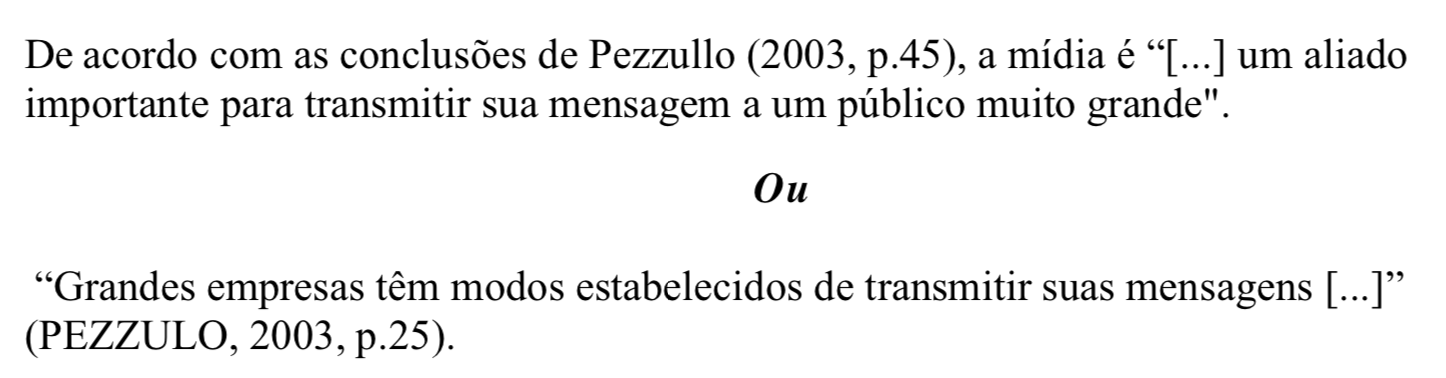
\includegraphics[height=4cm, width = 10cm]{./pic/diretamenos3linhas.png}
			\caption{Citação direta com menos de 3 linhas}
			\author{Guia de formatação SENAC }
			\label{fig_citacaodiretamenos3linhas}
		\end{figure}
	\end{block}
\end{frame}

\begin{frame}	
	\begin{block}{Citações Diretas}	
		 \begin{figure}[!htb]
			\centering	  				
			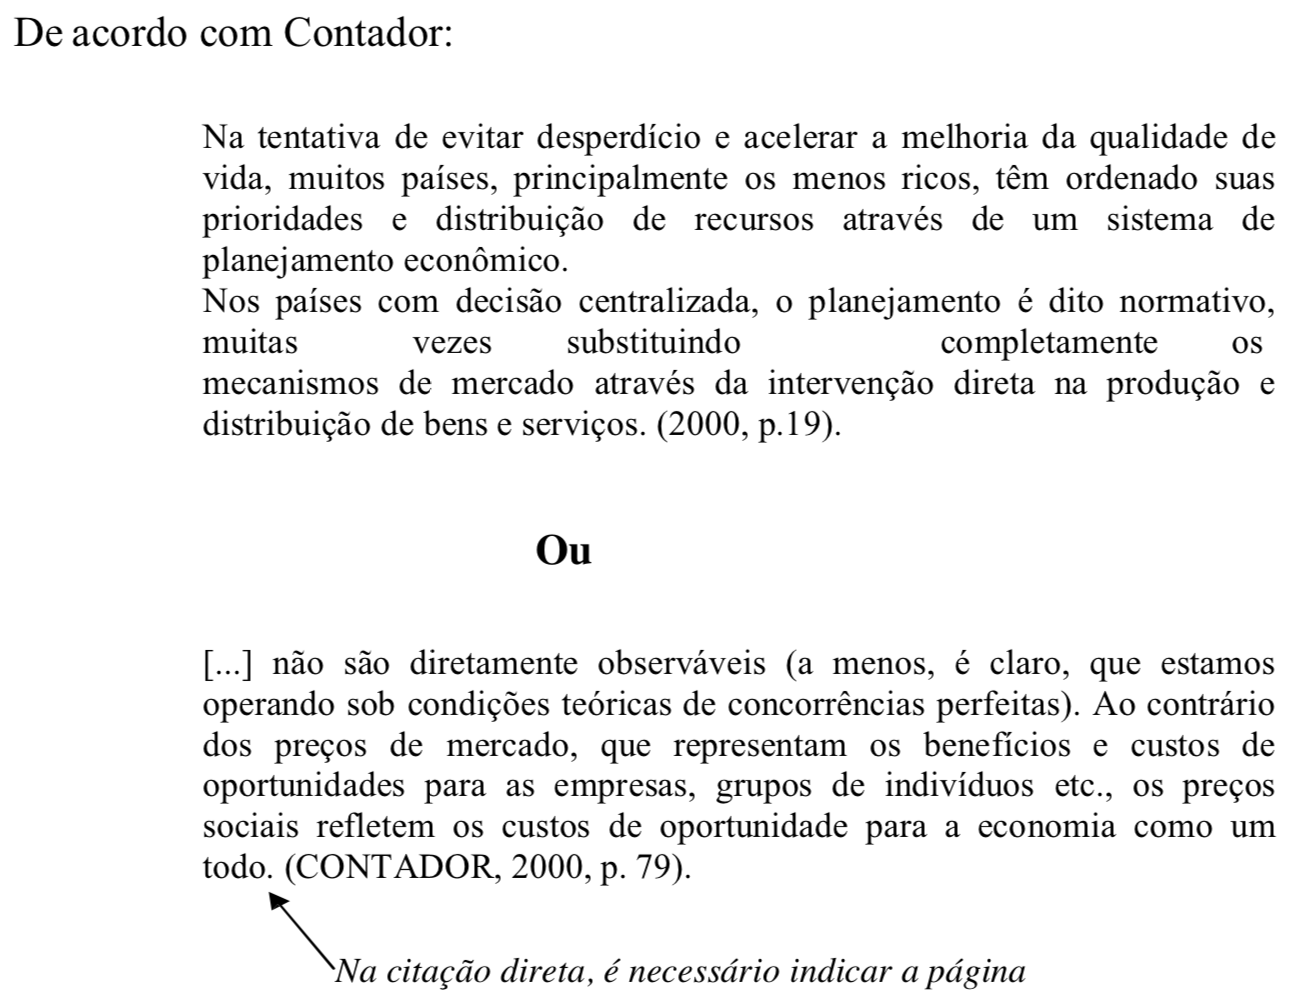
\includegraphics[height=7cm, width = 11cm]{./pic/diretamais3linhas.png}
			\caption{Citação direta com mais de 3 linhas}
			\author{Guia de formatação SENAC }
			\label{fig_citacaodiretamais3linhas}
		\end{figure}
	\end{block}
\end{frame}

\begin{frame}	
	\begin{block}{Citações Indiretas}	
		\begin{itemize}
			\item Aqui é reproduzida a idéia da fonte citada e não uma transcrição literal das frases
			\item Dispensa o uso de aspas duplas
			\item Dispensa a indicação da página
		\end{itemize}
	\end{block}
\end{frame}

\begin{frame}	
	\begin{block}{Citações Indiretas}	
		 \begin{figure}[!htb]
			\centering	  				
			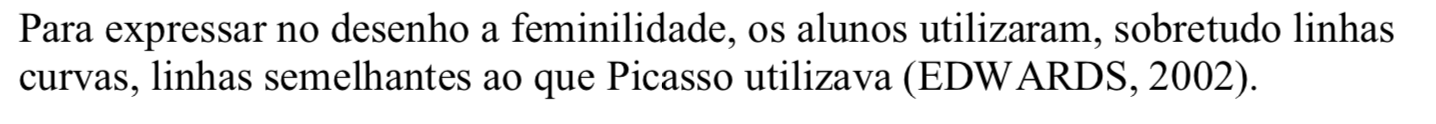
\includegraphics[height=2cm, width = 10cm]{./pic/citacaoindireta.png}
			\caption{Citação indireta}
			\author{Guia de formatação SENAC }
			\label{fig_citacaoindireta}
		\end{figure}
	\end{block}
\end{frame}

\begin{frame}	
	\begin{block}{Citações de Citações}	
		\begin{itemize}
			\item Citação direta ou indireta de texto que não temos acesso integral
		\end{itemize}
	\end{block}
\end{frame}

\begin{frame}	
	\begin{block}{Citações de Citações}	
		 \begin{figure}[!htb]
			\centering	  				
			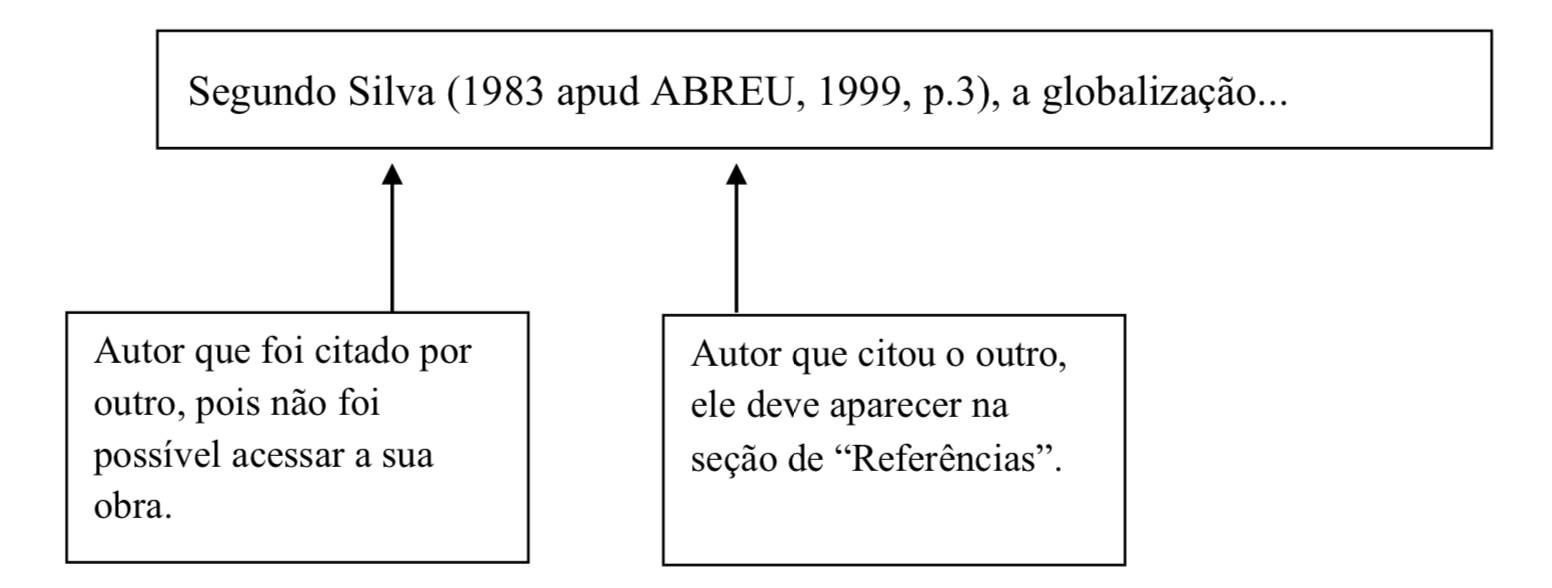
\includegraphics[height=5cm, width = 10cm]{./pic/apud.png}
			\caption{Citação de citação}
			\author{Guia de formatação SENAC }
			\label{fig_citacaodecitacao}
		\end{figure}
	\end{block}
\end{frame}

\begin{frame}	
	\begin{block}{Citações de vários trabalhos}	
		\begin{itemize}
			\item Vários autores sendo citados devem ser separados pelo critério auto-data
			\item Serguir ordem alfabética ou cronológica (Manter a ordem escolhida no texto todo!)
		\end{itemize}
	\end{block}
\end{frame}

\begin{frame}	
	\begin{block}{Citações de vários trabalhos}	
		 \begin{figure}[!htb]
			\centering	  				
			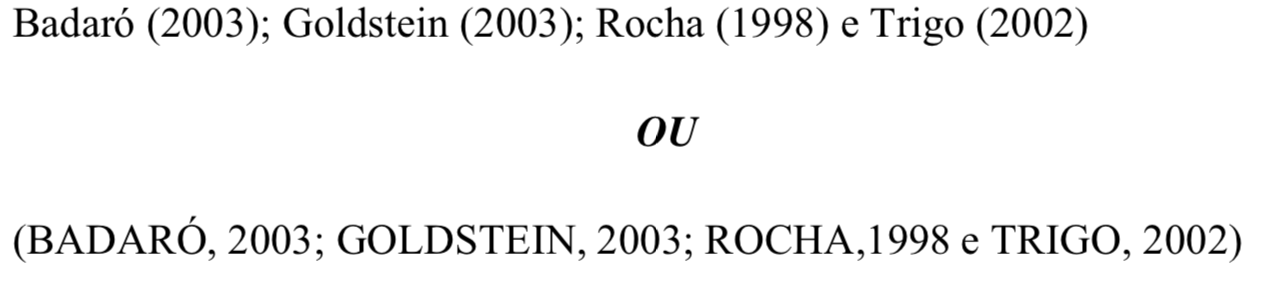
\includegraphics[height=3cm, width = 7cm]{./pic/alfabetica.png}
			\caption{Citações de vários trabalhos: ordem alfabética}
			\author{Guia de formatação SENAC }
			\label{fig_citacaodecitacao}
		\end{figure}
	\end{block}
	
\end{frame}

\begin{frame}	
	\begin{block}{Citações de vários trabalhos}	
		 \begin{figure}[!htb]
			\centering	  				
			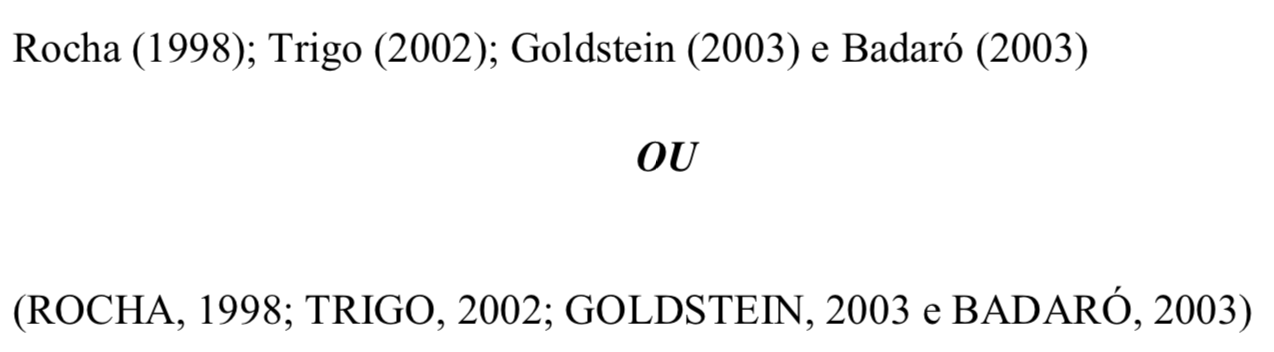
\includegraphics[height=3cm, width = 7cm]{./pic/cronologica.png}
			\caption{Citações de vários trabalhos: ordem cronológica}
			\author{Guia de formatação SENAC }
			\label{fig_citacaodecitacao}
		\end{figure}
	\end{block}
\end{frame}

\begin{frame}	
	\begin{block}{Citações de vários trabalhos do mesmo autor}	
	Trabalhos de mesmo autor com mesmo ano devem ser diferenciados pelo acréscimo de letras na citação.
		 \begin{figure}[!htb]
			\centering	  				
			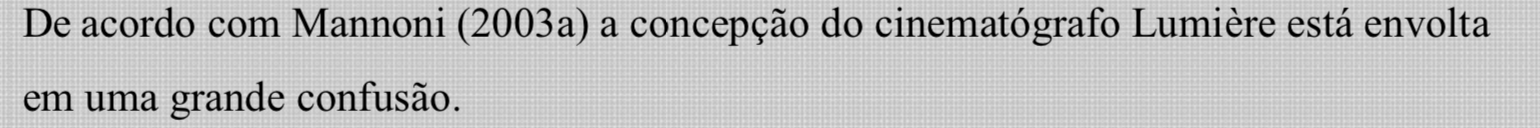
\includegraphics[height=1cm, width = 7cm]{./pic/letra.png}
			\caption{Citações de vários trabalhos: mesmo autor, mesmo ano}
			\author{Guia de formatação SENAC }
			\label{fig_citacaodecitacao}
		\end{figure}
	\end{block}
\end{frame}

\begin{frame}	
	\begin{block}{Sistema autor-data}	
		\begin{itemize}
			\item Sobrenome do autor e data de publicação entre parênteses
		\end{itemize}
	\end{block}
\end{frame}

\begin{frame}	
	\begin{block}{Sistema autor-data}	
	Trabalhos de mesmo autor com mesmo ano devem ser diferenciados pelo acréscimo de letras na citação.
		 \begin{figure}[!htb]
			\centering	  				
			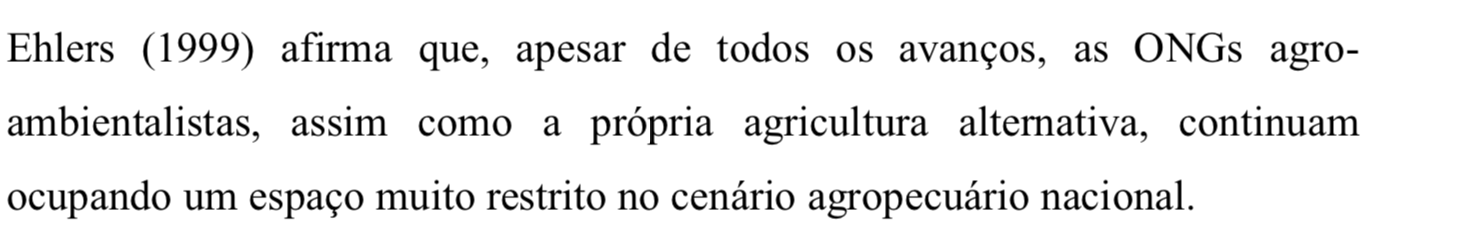
\includegraphics[height=1cm, width = 7cm]{./pic/autordata.png}
			\caption{Referência autor-data}
			\author{Guia de formatação SENAC }
			\label{fig_citacaodecitacao}
		\end{figure}
	\end{block}
\end{frame}

\begin{frame}	
	\begin{block}{Sistema numérico}	
		\begin{itemize}
			\item Citação única de algarismos arábicos, consecutivos que remetem a ordem dos trabalhos apresentados na referência
		\end{itemize}
	\end{block}
\end{frame}

\begin{frame}	
	\begin{block}{Sistema numérico}	
		 \begin{figure}[!htb]
			\centering	  				
			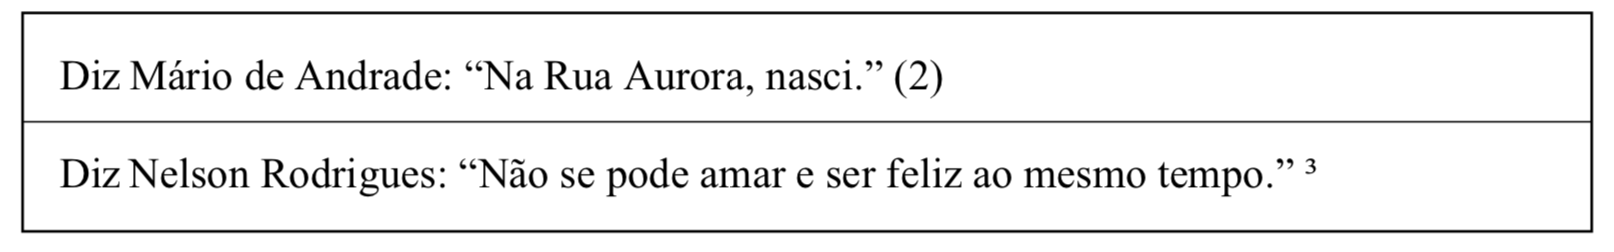
\includegraphics[height=1cm, width = 7cm]{./pic/numerico.png}
			\caption{Referência numérica}
			\author{Guia de formatação SENAC }
			\label{fig_citacaodecitacao}
		\end{figure}
	\end{block}
\end{frame}